\chapter{Evaluations} \label{ch:result}
The INTERACTION Dataset \footnote{https://interaction-dataset.com/} is used to compare the algorithms and models for tracking traffic participants. The dataset contains multiple scenarios in different locations captured using drones or fixed camera over variable amount of time. Each scenario consists of multiple traffic participants, identified by an ID, and each frame per 0.1s has a set of vehicles and their position and velocity in the x and y direction. Over different videos, the location with video of maximum length, 259.43 minutes, is chosen for this paper. There are 60 recorded files in this location with a total of 10,518 vehicles. The position for the vehicles in the x and y-direction is used as a measurement input to the algorithms, whereas the velocity in the x and y-direction is used to calculate the error and evaluate the estimates.The initial state of the system is set using assignments \eqref{eq:initial}.
\begin{equation}
\label{eq:initial}
\begin{split}
x_0 &= zonotope([zeros(n), diag([1000;1000;10;10;10;10])])\\
w_k &= [0.1;0.1;0.4;0.4;0.1;0.1]\\
v_k &= [0.1;0.1]
\end{split}
\end{equation}

\section{Computation Time}
\begin{figure}[htbp]
\centering
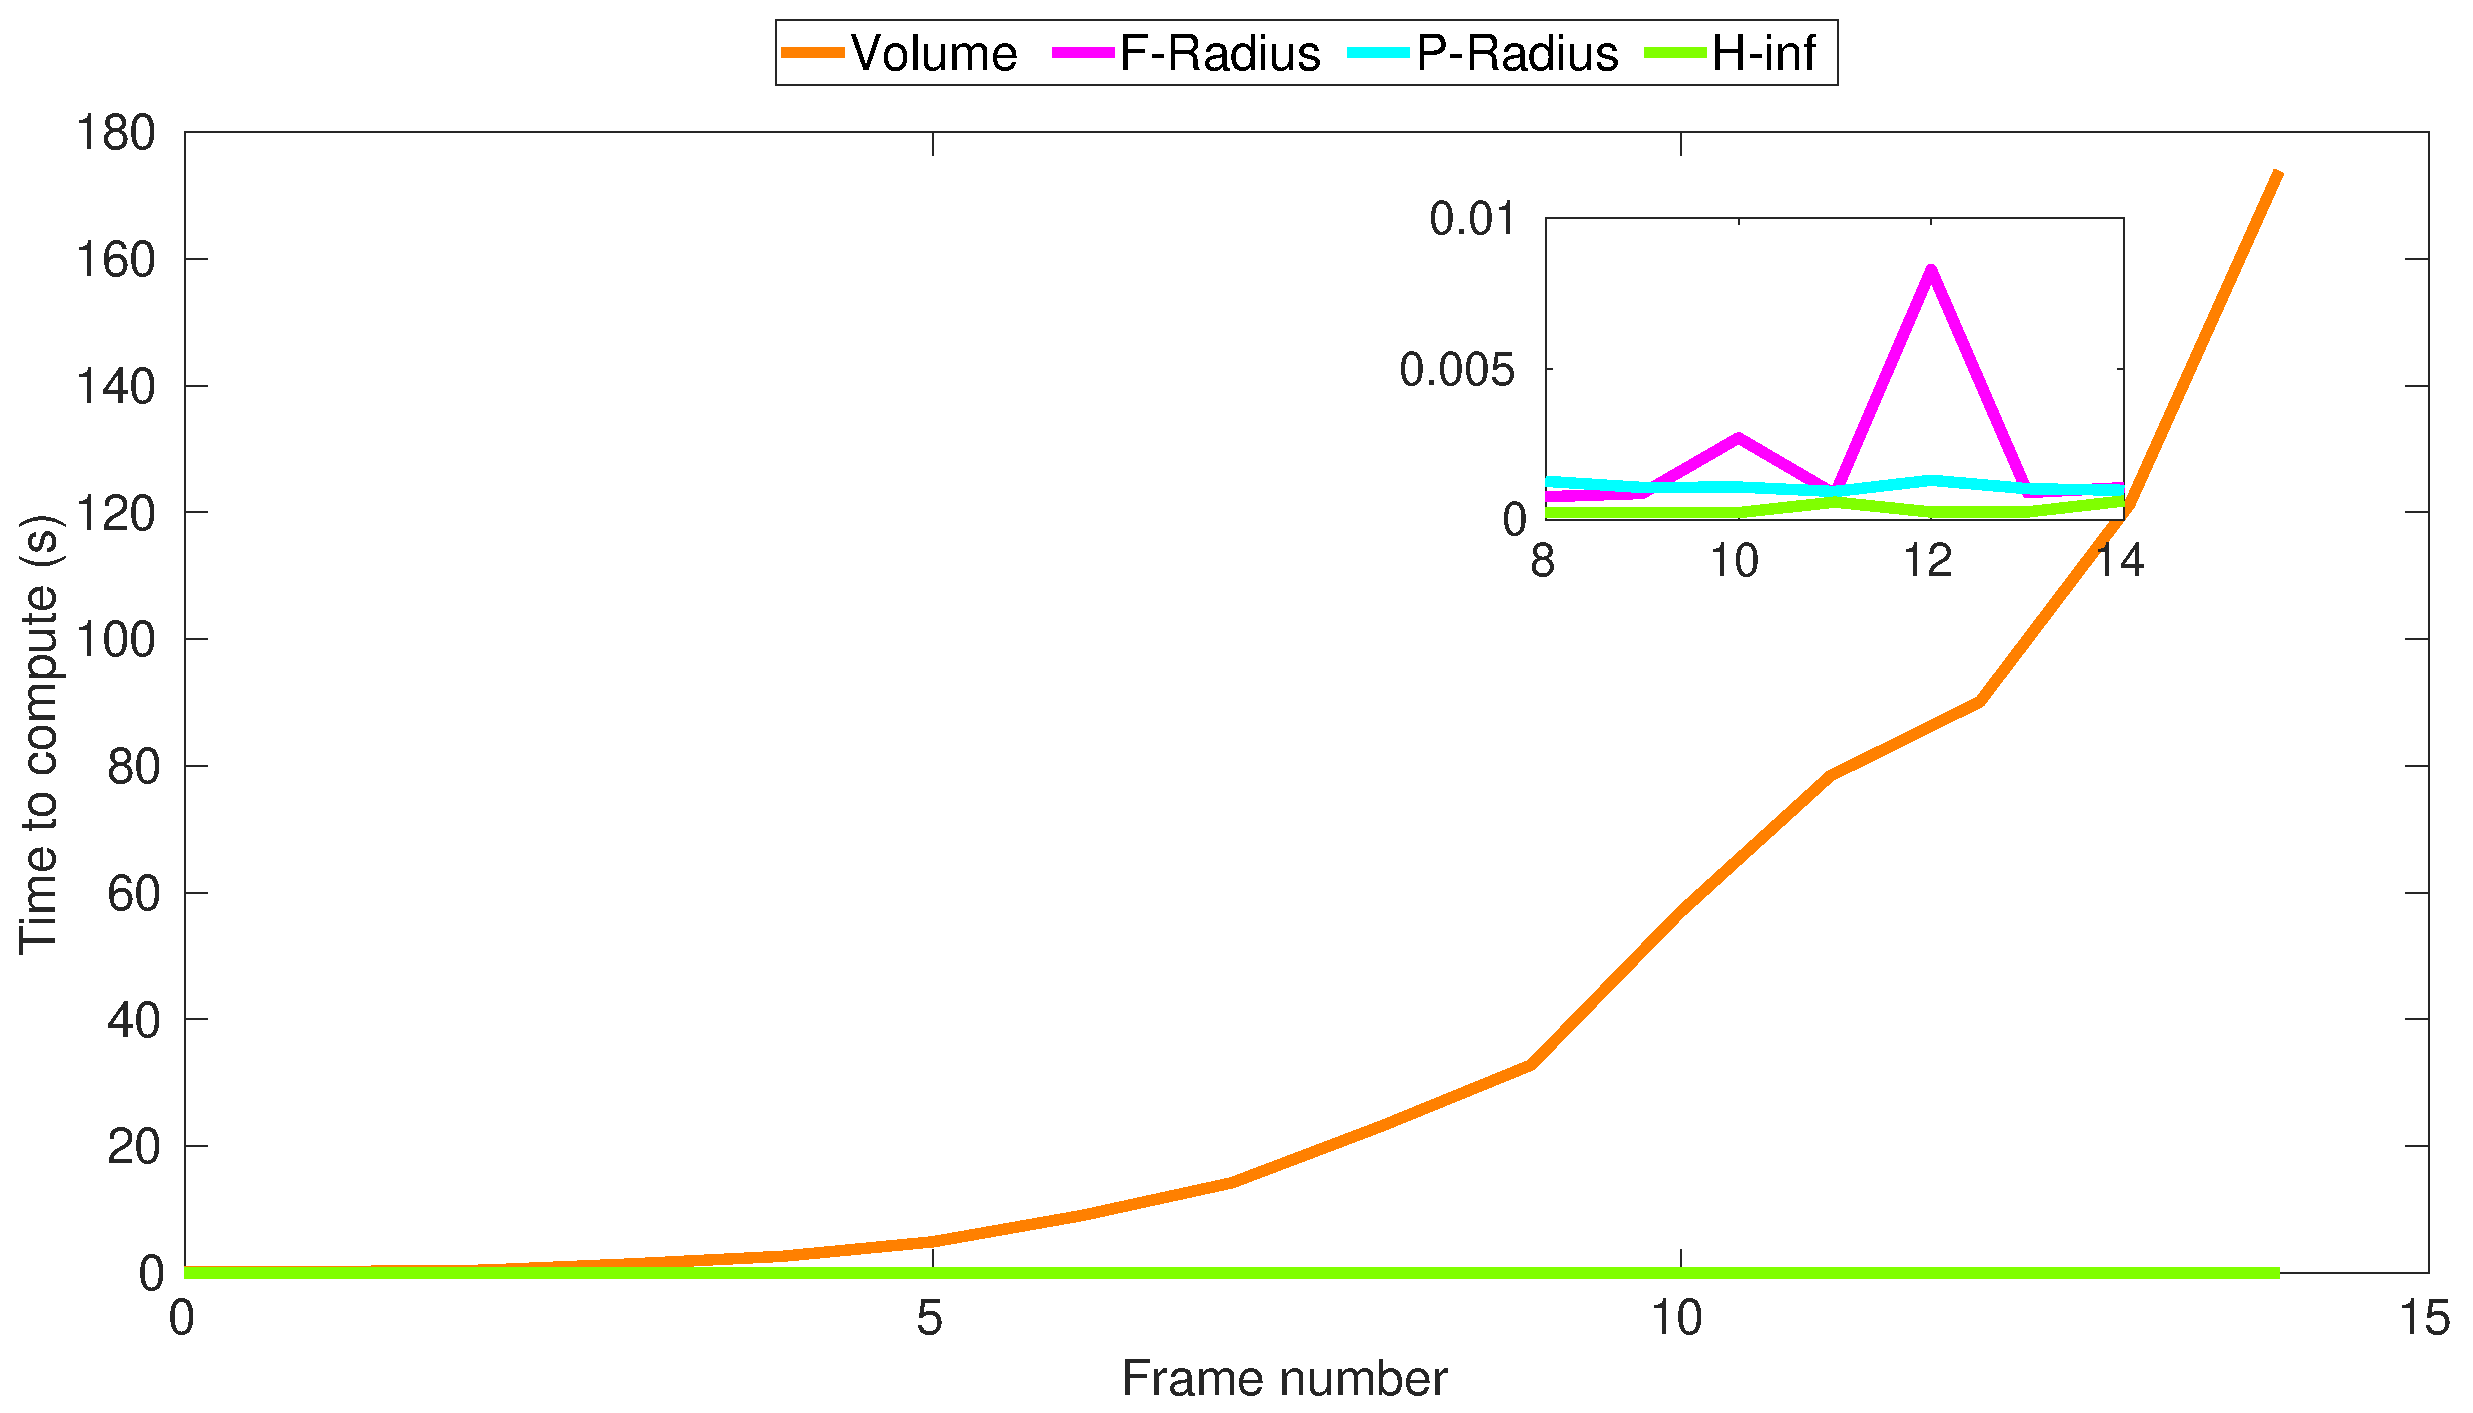
\includegraphics[width=\linewidth]{figures/timegraphh}
\caption{Computation time for each method to estimate using Constant Velocity Model}
\label{fig:timegraph}
\end{figure}

\begin{table}[htbp]
\caption{Comparison of computation time (ms) using Constant Velocity Model\\}
	\centering
	\renewcommand{\arraystretch}{1.1}
	\small	
	\begin{tabular}{l l}
		\toprule 
		\textbf{Method} & \textbf{Average Computation Time (ms)}\\ \midrule
		%-------------------------------------		
		F-Radius & 0.375\\
		P-Radius &0.319\\
		H-$\infty$ approximation & 0.147\\
		%--------------------------------------		
		\bottomrule
	\end{tabular}
	\label{tab:comptime}
\end{table}
Figure \ref{fig:timegraph} shows that computation time for Volume Minimization rises exponentially making it futile in the state estimation for collision avoidance system. On the contrary, Table \ref{tab:comptime} shows that the computation time for the other methods are negligible compared to the frame rate, i.e 100ms. Furthermore, the interval observer using H-$\infty$ has almost half the time required for the segment intersection methods, although the computation time does not consider the time for pre-computation for the techniques.



\section{Time to Converge}
\begin{table}[htbp]
\caption{Comparison of average time(in ms) to converge for unmeasured state\\}
	\centering
	\renewcommand{\arraystretch}{1.1}
	\small	
	\begin{tabular}{l l l l}
		\toprule 
		\textbf{Method} & \textbf{Constant Velocity} & \textbf{Constant Acceleration} & \textbf{Point Mass Model} \\ \midrule
		%-------------------------------------		
		F-Radius & 30 & 50 & 22\\
		P-Radius & 32 & 45 & 35\\
		H-$\infty$ approximation & 24 & 50 & 35\\
		%--------------------------------------		
		\bottomrule
	\end{tabular}
	\label{tab:convtime}
\end{table}
Table \ref{tab:convtime} compares the time for each of the technique to converge unmeasured state(velocity for constant velocity, acceleration for the rest). Segment Intersection using F-Radius works the best using Point Mass Model, as it converges the fastest.


Section \ref{eresult:setest} in the Extended Result Chapter shows the estimated bounds for all the models on a vehicle with varying acceleration. On comparing the estimation of velocity, same bounds are obtained from constant acceleration and point mass model, however, the bounds of acceleration from the latter is better than the former. Hence, point mass model is used to compare the algorithms for estimating acceleration on the following sections.


\section{Bounds}
\begin{table}[htbp]
\caption{Comparison of bounds of estimation\\}
	\centering
	\renewcommand{\arraystretch}{1.1}
	\small	
	\begin{tabular}{l l l l l l l}
		\toprule 
		& \multicolumn{6}{c}{\textbf{Constant Velocity}}\\
		\textbf{Method} & \textbf{$s_x$} & \textbf{$s_y$} & \textbf{$v_x$} & \textbf{$v_y$} & \textbf{$a_x$} & \textbf{$a_y$}\\ \midrule
		%-------------------------------------		
		F-Radius & .441 & .441 & 5.686 & 5.686 & - & -\\
		P-Radius & .4606 & .459 & 13.45 & 13.45 & - &	-\\
		H-$\infty$ approximation & .9867 &	.937 &	6.177 & 6.177 & - &-\\
		
		%--------------------------------------		
		
%		& \multicolumn{6}{c}{\textbf{Constant Acceleration}}\\
%		 & \textbf{$x$} & \textbf{$y$} & \textbf{$v_x$} & \textbf{$v_y$} & \textbf{$a_x$} & \textbf{$a_y$}\\ \midrule
%		%-------------------------------------		
%		F-Radius & .5713 &	.5075 &	8.461	& 8.461 &	15.86 &	15.97\\
%		P-Radius & .4598 &	.4523 &	16.39 &	16.39 &	16.61 &	17.42\\
%		H-$\infty$ approximation & 1.5 & 1.5 & 9.414 &	9.414 &	16.42 &	16.35\\
		
		%--------------------------------------		
		
%		& \multicolumn{6}{c}{\textbf{Singer Acceleration}}\\
%		 & \textbf{$x$} & \textbf{$y$} & \textbf{$v_x$} & \textbf{$v_y$} & \textbf{$a_x$} & \textbf{$a_y$}\\ \midrule
%		%-------------------------------------		
%		F-Radius &.4859	& .4859 &	7.38 & 7.383 &	11.53 &	11.53\\
%		P-Radius & .7035 &	.7035 &	23.23 &	23.23 &	10.23 &	10.23\\
%		H-$\infty$ approximation & 1.276 &	1.19 &	9.691 &	9.691 &	10.01 &	10.01\\
%		
%		%--------------------------------------		
		
		& \multicolumn{6}{c}{\textbf{Point Mass Model}}\\
		 & \textbf{$s_x$} & \textbf{$s_y$} & \textbf{$v_x$} & \textbf{$v_y$} & \textbf{$a_x$} & \textbf{$a_y$}\\ \midrule
		%-------------------------------------		
		F-Radius & .5713 &	.5075 &	8.461	& 8.461 &	15.79 &	15.78\\
		P-Radius & .4598 &	.4523 &	16.39 &	16.39 &	16.43 &	16.18\\
		H-$\infty$ approximation & 1.5 & 1.5 & 9.414 &	9.414 &	16.11 &	16.24\\
		\bottomrule
	\end{tabular}
	\label{tab:bound}
\end{table}
Bounds using constant velocity model is tighter compared to point mass model as seen from Table \ref{tab:bound}. The segment intersection using F-Radius has the tighter bounds compared to the other techniques. Interesting to note, the H$-\infty$ has much higher bounds in the initial time steps.


\section{Accuracy}
Accuracy is represented by the root mean square error(RMSE) of the estimation from the true state of the system. Since, the dataset does not have measurement for acceleration, the accuracy of acceleration cannot evaluated.

The initial estimation before convergence gives extreme error which affetc the result, hence the estimation after convergence(i.e. after 50 time steps) are allowed in the evaluation. The RMSE is then computed as a percentage from the maximum measurement in the time frame.

The boxplot of RMSE using measurements in velocity in x direction using Point Mass Model for all the techniques are shown in Figure \ref{fig:boxplot}. The segment minimization using P-Radius has high range of extremes and the mean error is also greater than the other methods. The range of error is the lowest for H-$\infty$ observer with mean 
1.9048 and standard deviation of 1.9776 for $velocity_x$. Detailed report of mean and standard deviation of each of the method can be found in table \ref{tab:errormean}. The error expectation from segment minimization from F-Radius is similar to H-$\infty$ observer, however, the error in measured state is slightly lesser in F-Radius compared to H-$\infty$ observer.
\begin{figure}[h]
\centering
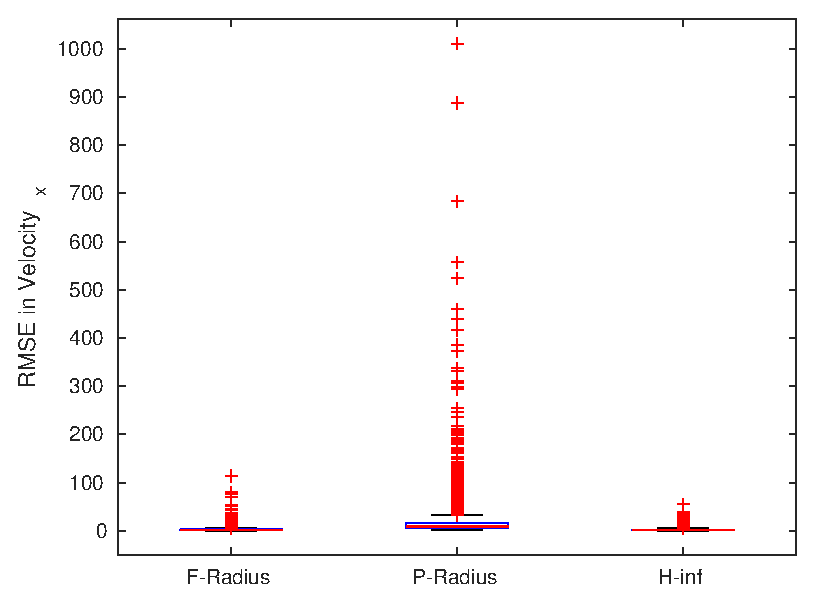
\includegraphics[width=\linewidth]{figures/Error/boxplotall}
\caption{RMSE(Root Mean Squared Error)}
\label{fig:boxplot}
\end{figure}

\begin{table}[htbp]
\caption{Comparison of RMSE}
	\centering
	\renewcommand{\arraystretch}{1.1}
	\small	
	\begin{tabular}{l l l l l}
		\toprule 
		& \multicolumn{4}{c}{\textbf{Mean $\pm$ SD}} \\ \cmidrule{2-5}
		\textbf{Method} & \textbf{$s_x$} & \textbf{$s_y$} & \textbf{$v_x$} & \textbf{$v_y$}\\ \midrule
		%-------------------------------------		
		F-Radius & $0.0007\pm 0.0004$ &  $0.0004  \pm 0.0003$ &  $2.3412 \pm 2.7092$ &   $2.4184 \pm 1.5641$ \\
		P-Radius & $0.0016 \pm 0.0020$ &   $0.0008 \pm 0.0017$  & $13.4470 \pm 26.2465$ &  $13.7642 \pm 54.6724$\\
		H-$\infty$ approximation & $0.0007 \pm 0.0004$ &  $0.0006 \pm 0.0005$   & $1.9048 \pm  1.9776$  &  $ 2.1230 \pm  2.1946$\\
		%--------------------------------------		
		\bottomrule
	\end{tabular}
	\label{tab:errormean}
\end{table}

%Time comparison for each method for n vehicles is shown in figure [cite]
%
%As seen from Fig. \ref{fig:segmentminimization}, the upper and lower bounds of the state estimation by Segment Intersection(using Frobenius norm) of the system bounds the true state. Comparing the error in different states of the system, as shown in Fig. \ref{fig:comparison}, suggests that all the algorithms require around 1s to converge to near the true state. Interesting to note, the Interval Estimation has a higher error peak compared to Segment Minimization using the same dataset.\\
%
%The Fig. \ref{fig:histogram} shows the Histogram of RMSE (Root Mean Square Error) of estimation from Segment Minimization. The errors are calculated after 10 seconds in order to avoid the initial peak. The histograms suggest that, the method gives little error for estimating the measured state, whereas, for unmeasured state like velocity, the error is at most twice the true state.


%\begin{figure}[h!]
%\begin{subfigure}{.5\textwidth}
%\centering
%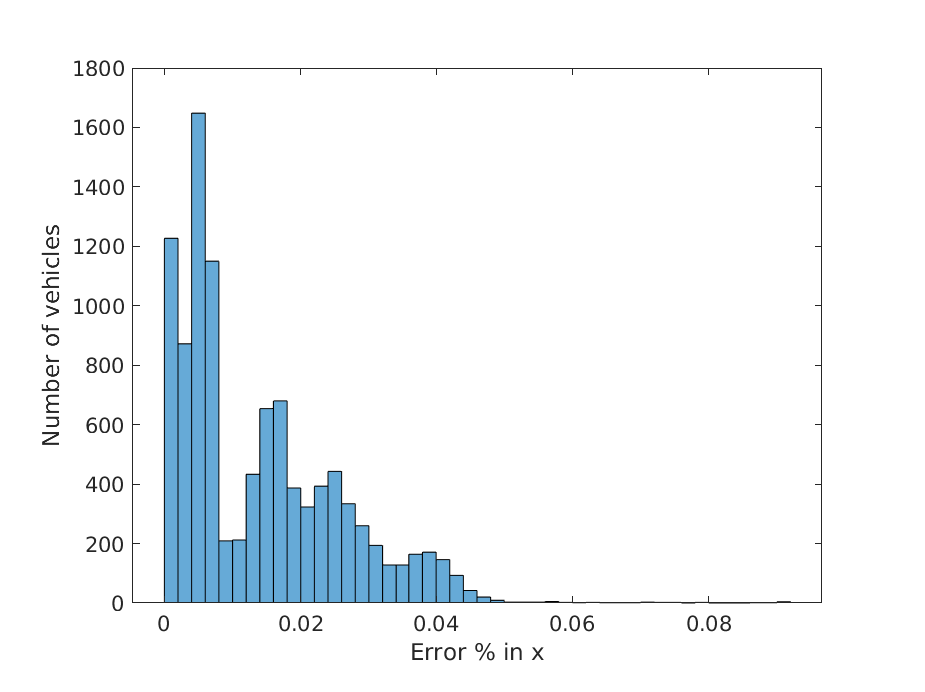
\includegraphics[width=.8\linewidth]{figures/s_caXerror}
%\caption{RMSE $x$}
%\end{subfigure}
%\begin{subfigure}{.5\textwidth}
%\centering
%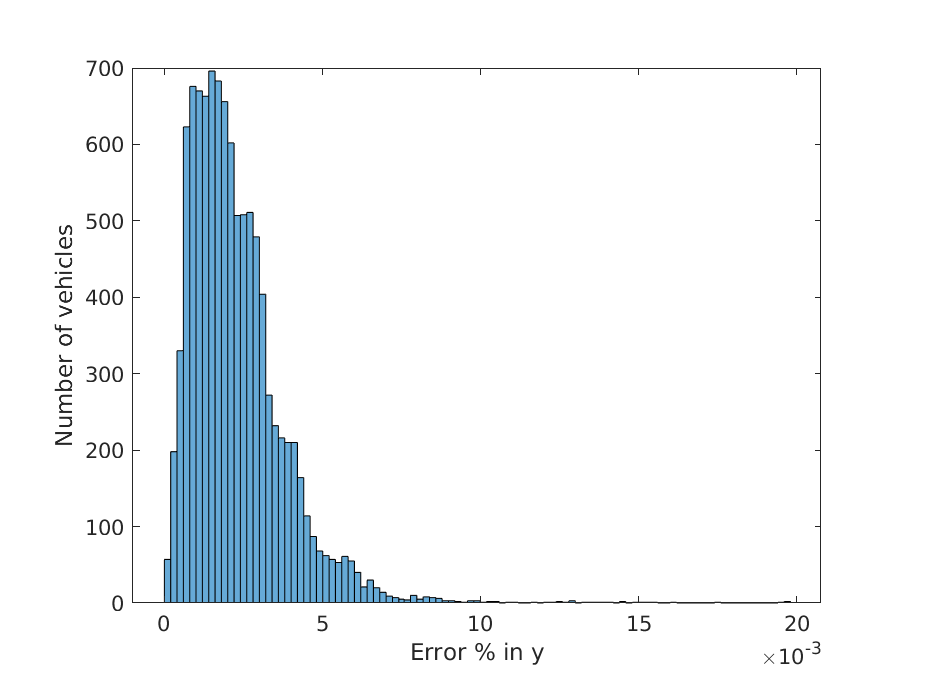
\includegraphics[width=.8\linewidth]{figures/s_caYerror}
%\caption{RMSE $y$}
%\end{subfigure}
%\begin{subfigure}{.5\textwidth}
%\centering
%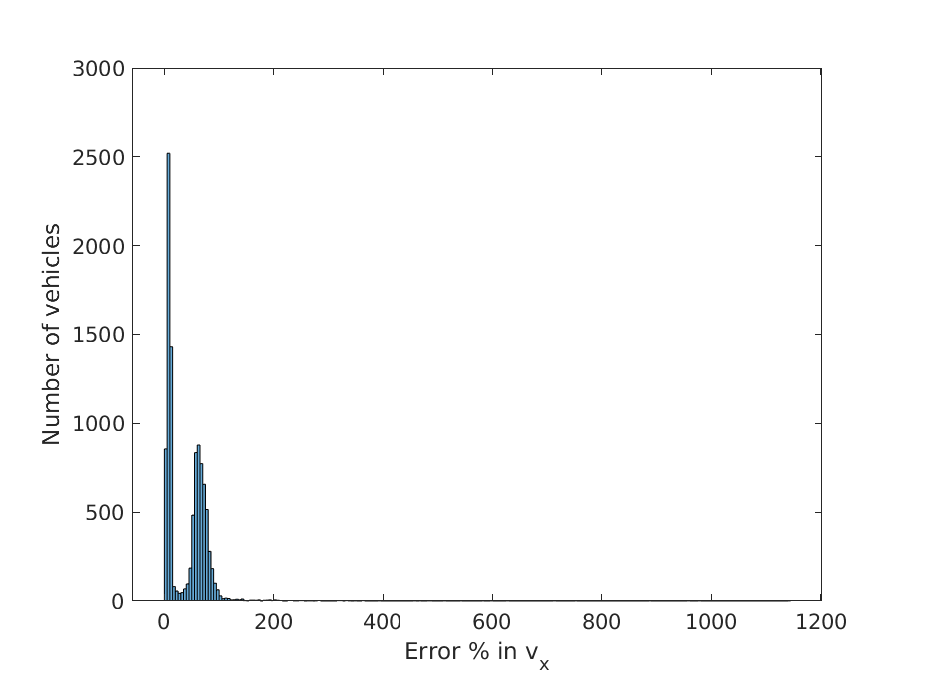
\includegraphics[width=.8\linewidth]{figures/s_cavXerror}
%\caption{RMSE in $velocity_x$}
%\end{subfigure}
%\begin{subfigure}{.5\textwidth}
%\centering
%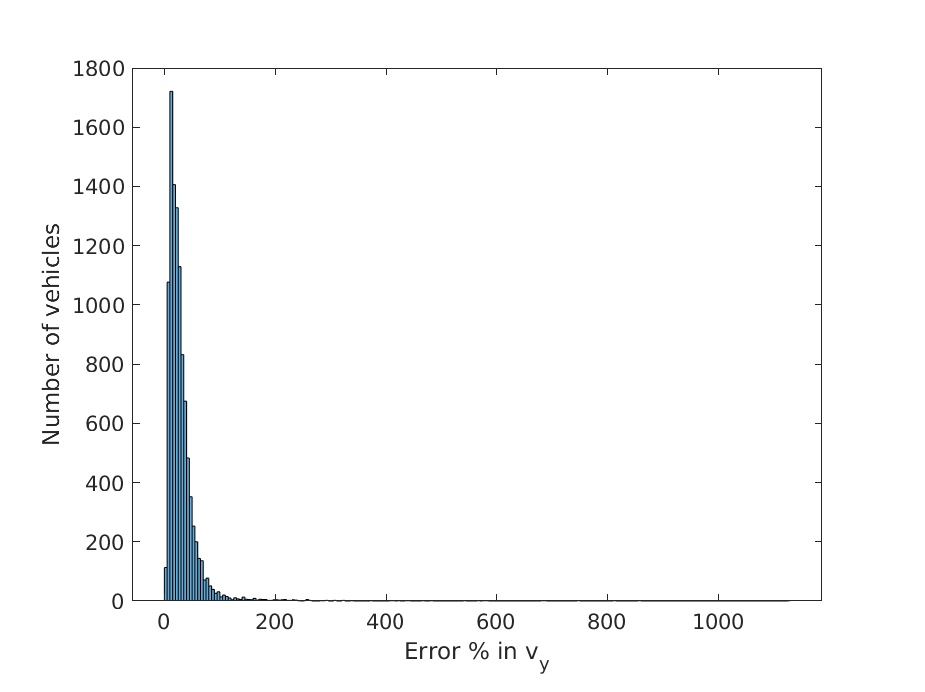
\includegraphics[width=.8\linewidth]{figures/s_cavYerror}
%\caption{RMSE in $velocity_y$}
%\end{subfigure}
%\caption{Histogram of errors from Segment Minimizer on 651 vehicles }
%\label{fig:histogram}
%\end{figure}
%\begin{itemize}
%\item{Efficiency}
%\item{Accuracy}
%\item{Performance Metric}
